\documentclass[../notes.tex]{subfiles}

\pagestyle{main}
\renewcommand{\chaptermark}[1]{\markboth{\chaptername\ \thechapter\ (#1)}{}}
\setcounter{chapter}{6}

\begin{document}




\chapter{Presentations}
\section{Day 1 (1-6)}
\begin{itemize}
    \item \marginnote{3/11:}Nate's presentation.
    \begin{itemize}
        \item Figure out what IC\textsubscript{50} means, and why nanomolar (including single-digit) is good!
        \item Explain bio terms (but I'm already planning this).
        \begin{itemize}
            \item Make sure I have oncometabolite definition right!
        \end{itemize}
        \item Make sure all mechanistic/synthetic details are right and explainable (but I'm already planning this).
        \begin{itemize}
            \item "You should be able to right a mechanism for any reaction you're going to present" - Steve.
            \item "If you're in a job interview, you have to be able to have some answer if someone asks how the reaction goes."
            \item "Sometimes I know and sometimes I don't, and then I have to look up a bunch of papers. And then sometimes I can figure it out and sometimes I can't, but at least I have something to say then." Sweet!
        \end{itemize}
    \end{itemize}
    \item Steve to Dennis: "All of these presentations should have been downloaded ahead of time."
    \item Frank's (Harvard) presentation.
    \begin{itemize}
        \item Vadadustat.
        \item "Slow down, breathe, and don't read from the slide."
        \item "You gonna walk us through that scheme? Because otherwise, it's useless."
        \begin{itemize}
            \item Make sure I explain all figures, including crystal structures!! Learn the hydrogen bonds.
        \end{itemize}
        \item Make sure I can explain ambiguous selectivity, too!!
        \item \ce{HBr} works to hydrolyze \emph{activated} (e.g., phenyl) methyl ethers (and can do nitrile hydrolysis at the same time).
        \begin{itemize}
            \item Explain selectivity for chloro S\textsubscript{N}Ar on \emph{s}-triazene vs. \emph{ortho}-pyridine.
            \item More activated/under more mild conditions. Look up typical conditions for pyridine S\textsubscript{N}Ar and look to differentiate temperature, acid, etc. from the used conditions.
        \end{itemize}
    \end{itemize}
    \item Minh's presentation.
    \begin{itemize}
        \item Voydeya.
        \item Appreciating structural/retrosynthetic challenges is probably a good idea!
        \item Make sure I know what the biuret test is (a protein test --- like the functional group tests Steve discussed that day --- that does not contain biuret, but gives a positive result to the peptide-like bonds in biuret).
        \item Check timing: Make sure I get everything in in 10 minutes, and don't linger on the bio!
        \item Sleep well both of the next two nights!
    \end{itemize}
    \item Alexander's presentation.
    \begin{figure}[h!]
        \centering
        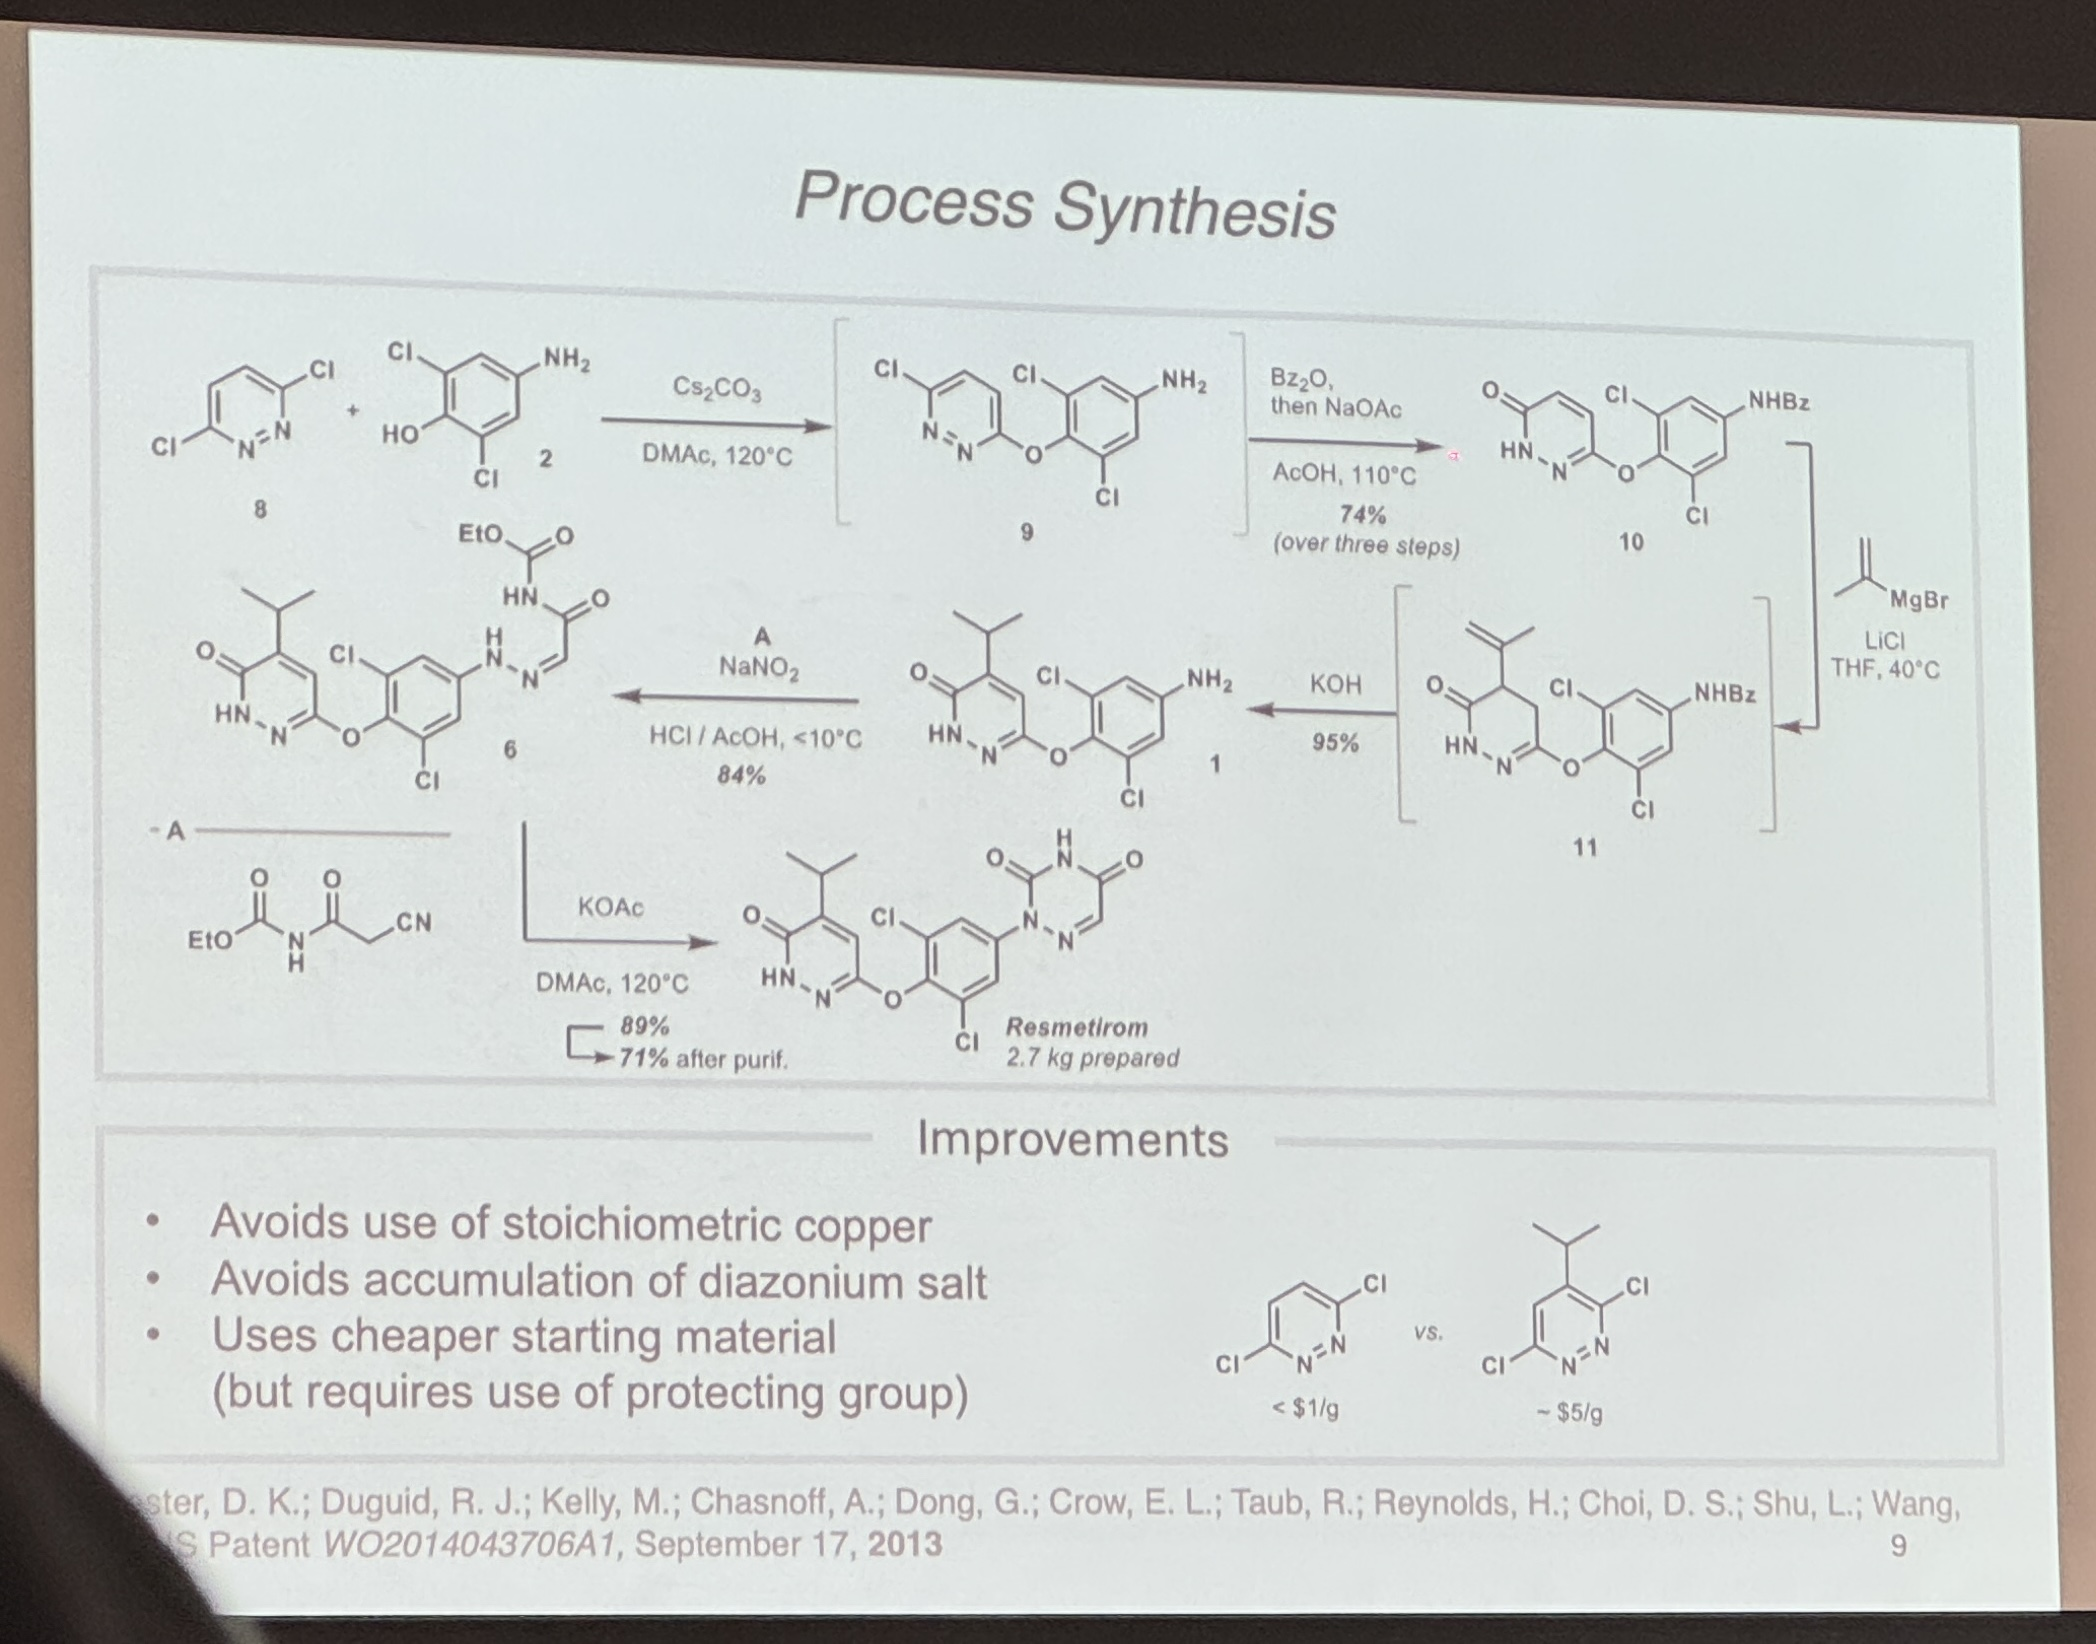
\includegraphics[width=0.7\linewidth]{PresAlexander.JPG}
        \caption{Alexander M\"{u}ller's graphic design.}
        \label{fig:PresAlexander}
    \end{figure}
    \begin{itemize}
        \item Resmetirom.
        \item Electron-rich arenes easily oxidize in the body, leading to redox cycling. Causes safety/toxidity issues.
        \begin{itemize}
            \item Good discussion of design principles; keep doing the same!
        \end{itemize}
        \item Good retrosynthesis, followed by synthesis.
        \item Dives into mechanisms of key steps.
        \item Good graphic design: Boxes. Very clean and clear. Citations in light grey at bottom left.
        \item Numbering chemicals and compounds is a good idea.
        \item Explaining selectivity is definitely needed!
    \end{itemize}
    \item Angel's presentation.
    \begin{itemize}
        \item Ceftobiprole: Staph antibiotic.
        \item Starts with retrosynthetic analysis of moieties.
        \item Gives a total nitrogen count; I could/should, too!
        \item Gives a discovery timeline.
        \item Know the mutations.
        \item Drawing out arrow-pushing mechanisms is not inappropriate.
        \item Make changes clear in large molecules moving from one to the next with colored bonds, as Steve does! Otherwise, you just get lost as to what's changing\dots
    \end{itemize}
    \item On Thursday, we'll start at 9:00 instead of 9:05.
    \item Kwanwoo's presentation.
    \begin{figure}[H]
        \centering
        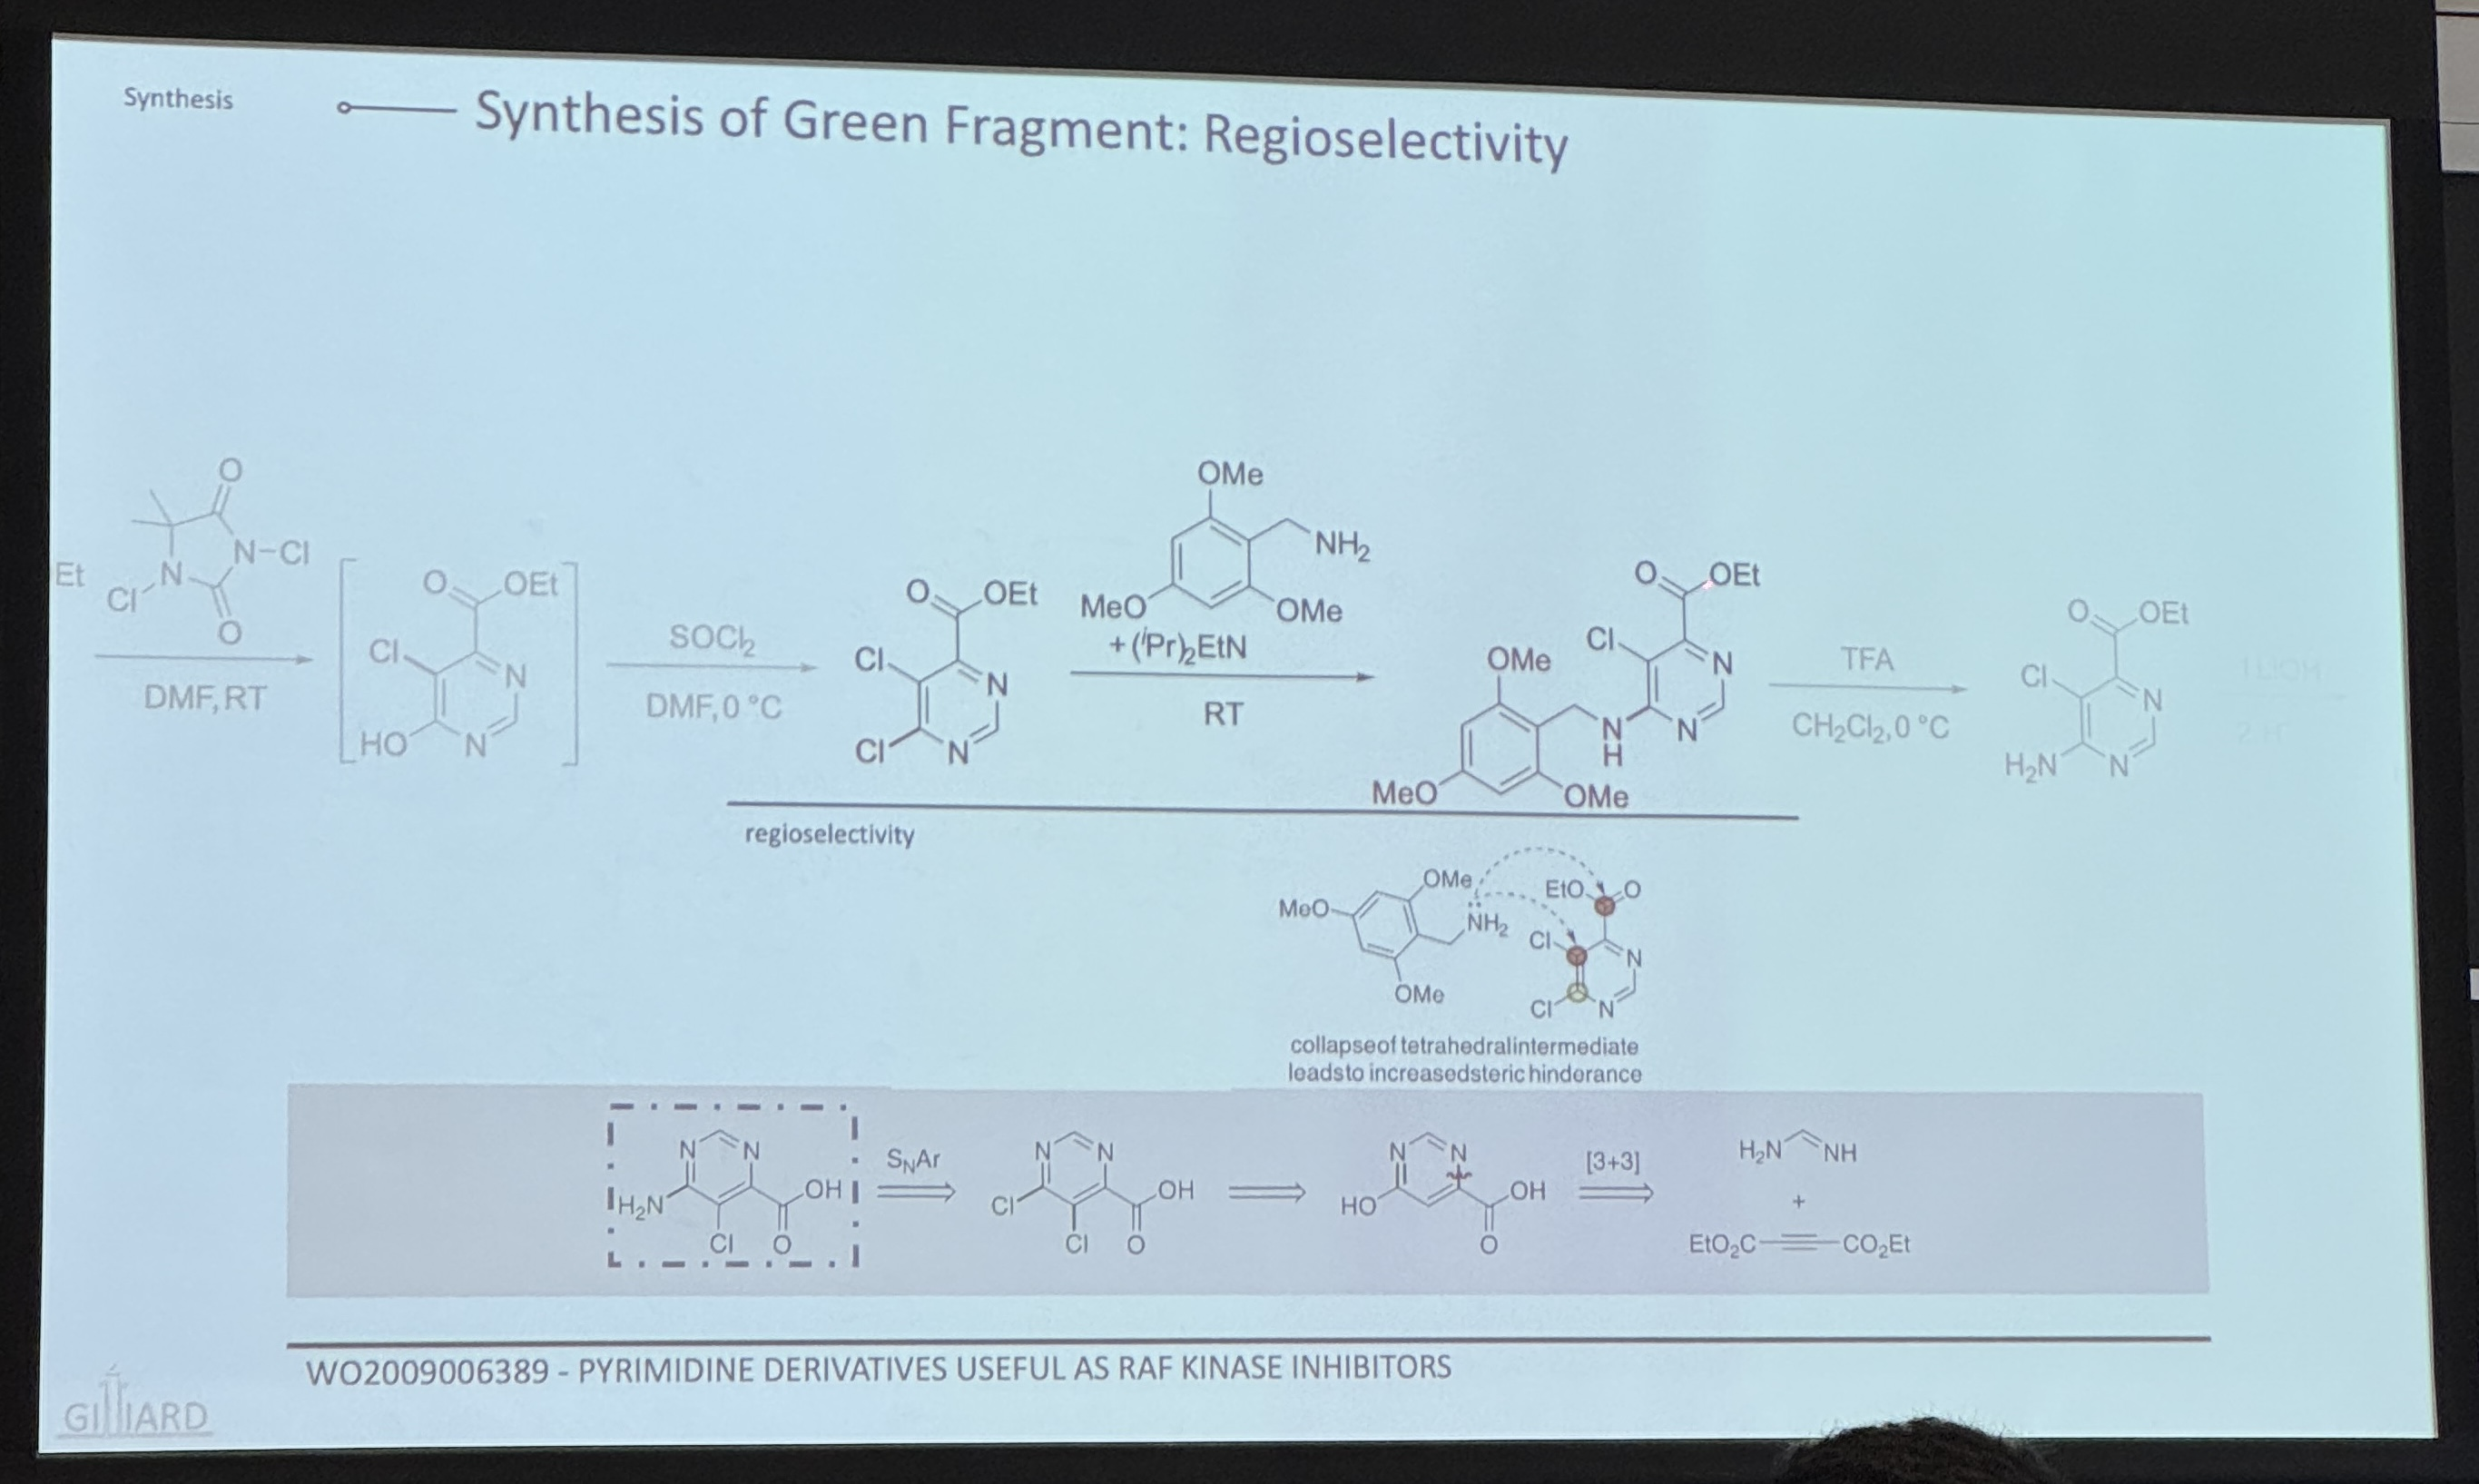
\includegraphics[width=0.7\linewidth]{PresKwanwoo.JPG}
        \caption{Kwanwoo Park's graphic design.}
        \label{fig:PresKwanwoo}
    \end{figure}
    \begin{itemize}
        \item Ojemda.
        \item Also uses MIT/Gilliard slide template!
        \item Also discussing a glioma; could give him a shoutout in my presentation!
        \item Slides are too cluttered and he's reading off the slides.
        \item Good retrosynthetic analysis. Color-codes fragments (using pastel-colored boxes might be better, then keeping them on each slide).
        \item Points out Hantzsch; I should make a fuss about names as well.
        \item Know the names of functional groups! Know the carbon numbering in my molecule.
        \item Graphic design.
        \begin{itemize}
            \item Mechanism in pop-up box is a good approach.
            \item Keeping the general scheme at the bottom of each slide, being progressively highlighted, as you move through bigger synthetic details up top.
            \item Chemoselectivity with circles in popup box.
        \end{itemize}
        \item Know reagent names, and functional group names.
    \end{itemize}
\end{itemize}



\section{Day 2 (7-14)}
\begin{itemize}
    \item \marginnote{3/13:}Jasmin's presentation.
    \begin{itemize}
        \item Xolremdi.
        \item Also does limitations of ok med chem synthesis!
        \item Does retrosynthetic analysis separately from forward synthesis; would have been a good idea, as Christine suggested.
        \item Uses a table beneath a larger, marked up scheme to show screened conditions for one reaction.
        \item "Silica gel pad" means filtration, not chromatography, which is why they can get away with it.
        \item Catalytic \ce{KI} and bulky base can do Finkelstein-type chloride/iodide exchange \emph{in situ} before S\textsubscript{N}2 displacement with the other reaction.
    \end{itemize}
    \item Yifan's presentation.
    \begin{figure}[H]
        \centering
        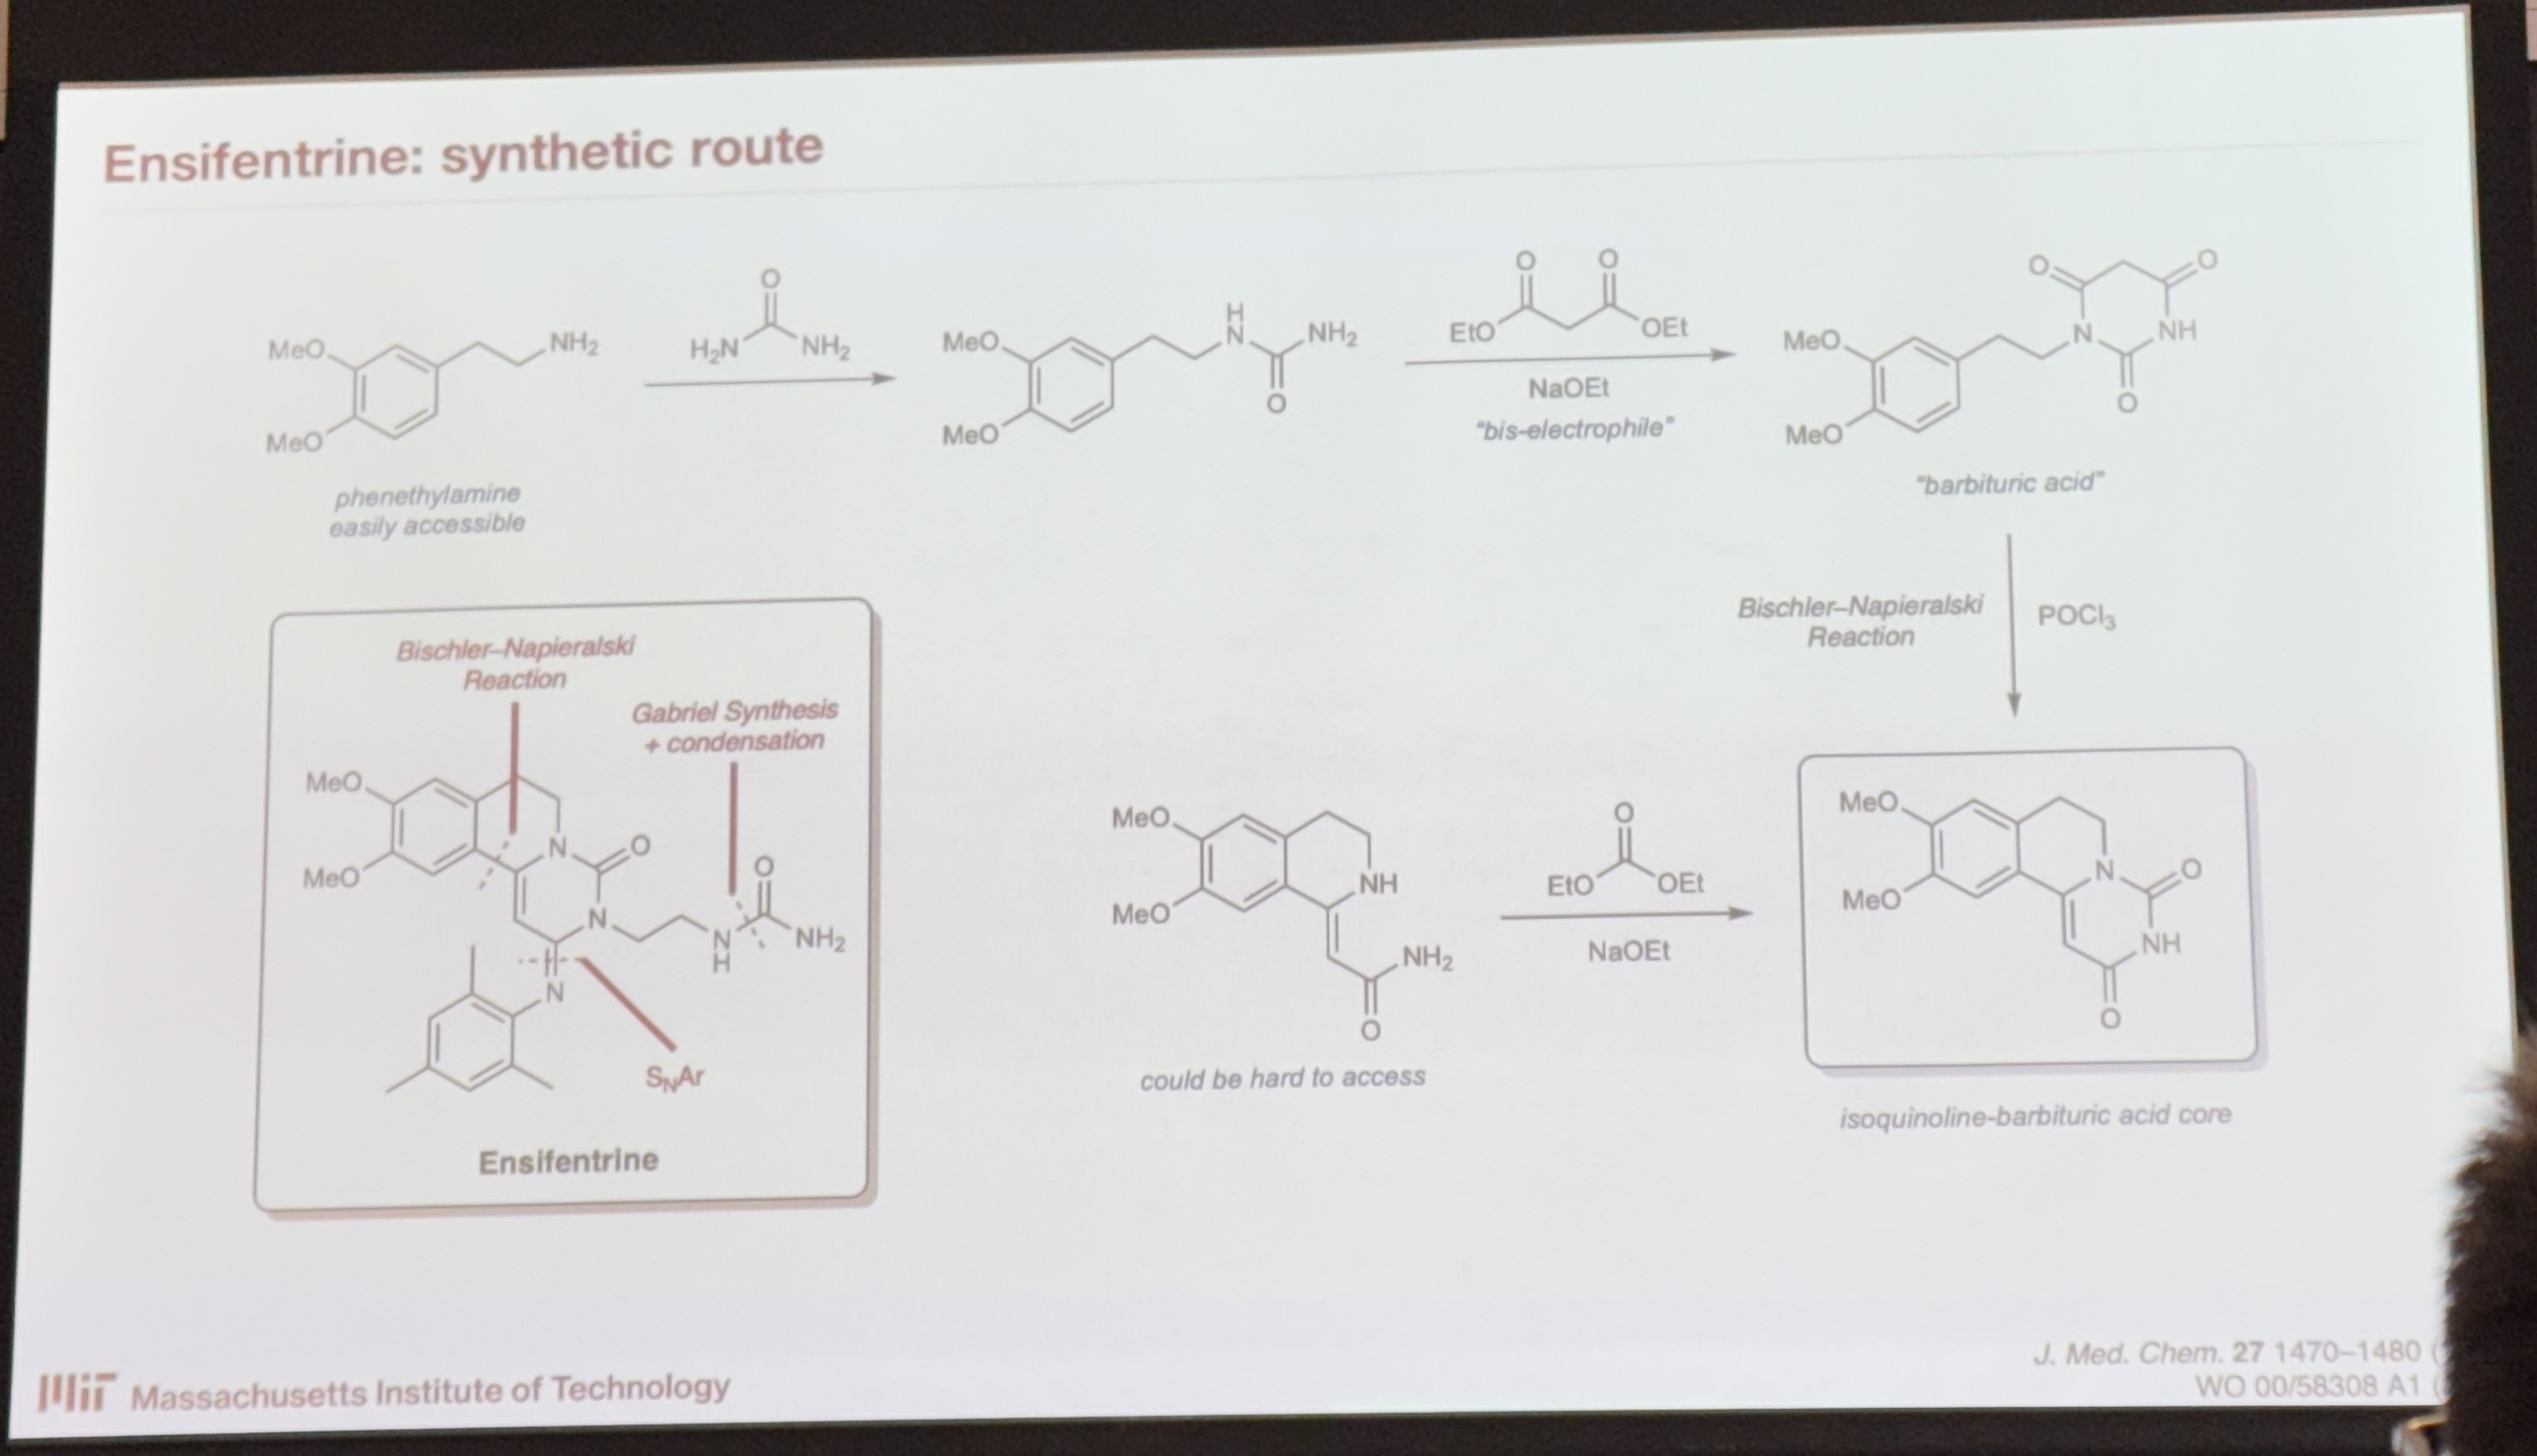
\includegraphics[width=0.7\linewidth]{PresYifan.JPG}
        \caption{Yifan's graphic design.}
        \label{fig:PresYifan}
    \end{figure}
    \begin{itemize}
        \item Emphasizing first-in-class and novel mechanisms of action may be a good idea.
        \item Graphic design: Disconnections labeled with reactions in a popup box!
        \item Finkelstein again: \ce{NaI}, \ce{K2CO3}, and 2-butanone (like W. S. Johnson!).
    \end{itemize}
    \item Yuzhe's presentation.
    \begin{itemize}
        \item Deyryxikutubub.
        \item Talks about mental health effects of having a disease, too!
        \item Numbering compounds with different numbers for different protecting groups (variables), as papers often do!
    \end{itemize}
    \item My presentation.
    \begin{itemize}
        \item \ce{C-F-O} bonds aren't really a thing; it's more of an interaction.
        \item We did actually talk about \emph{s}-triazines in class (oops); Steve made fun of the name.
        \item TFA, \ce{HC(OMe)3} is a common drying agent, an alternative to a Dean-Stark apparatus.
        \begin{itemize}
            \item Both things I put up are plausible, but drying is more common.
        \end{itemize}
        \item Steve points out that Cyanamid was acquired by another company, then bought by Pfizer (like everything else).
    \end{itemize}
    \item Jordan Bench's presentation.
    \begin{itemize}
        \item Lazertinib.
        \item Steve points out a number of things in the reactions that would be hard to tell from patents.
        \begin{itemize}
            \item Formate is for transfer hydrogenation.
        \end{itemize}
        \item Patent authors use patent generics a lot, because otherwise people will make a slight improvement, repatent, and sell more cheaply.
        \item You have to do a certain number of the examples in the patent in order to justify it, but not all of them.
    \end{itemize}
    \item Georgia's presentation.
    \begin{itemize}
        \item Miplyffa.
        \item Rare disease (only 300 people in the US), so test cases to justify the approval were only on 4-5 people.
        \item Process synthesis at \SI{50}{\gram} scale, but maybe that makes sense with the small number of people affected.
    \end{itemize}
    \item Elizabeth's presentation.
    \begin{figure}[H]
        \centering
        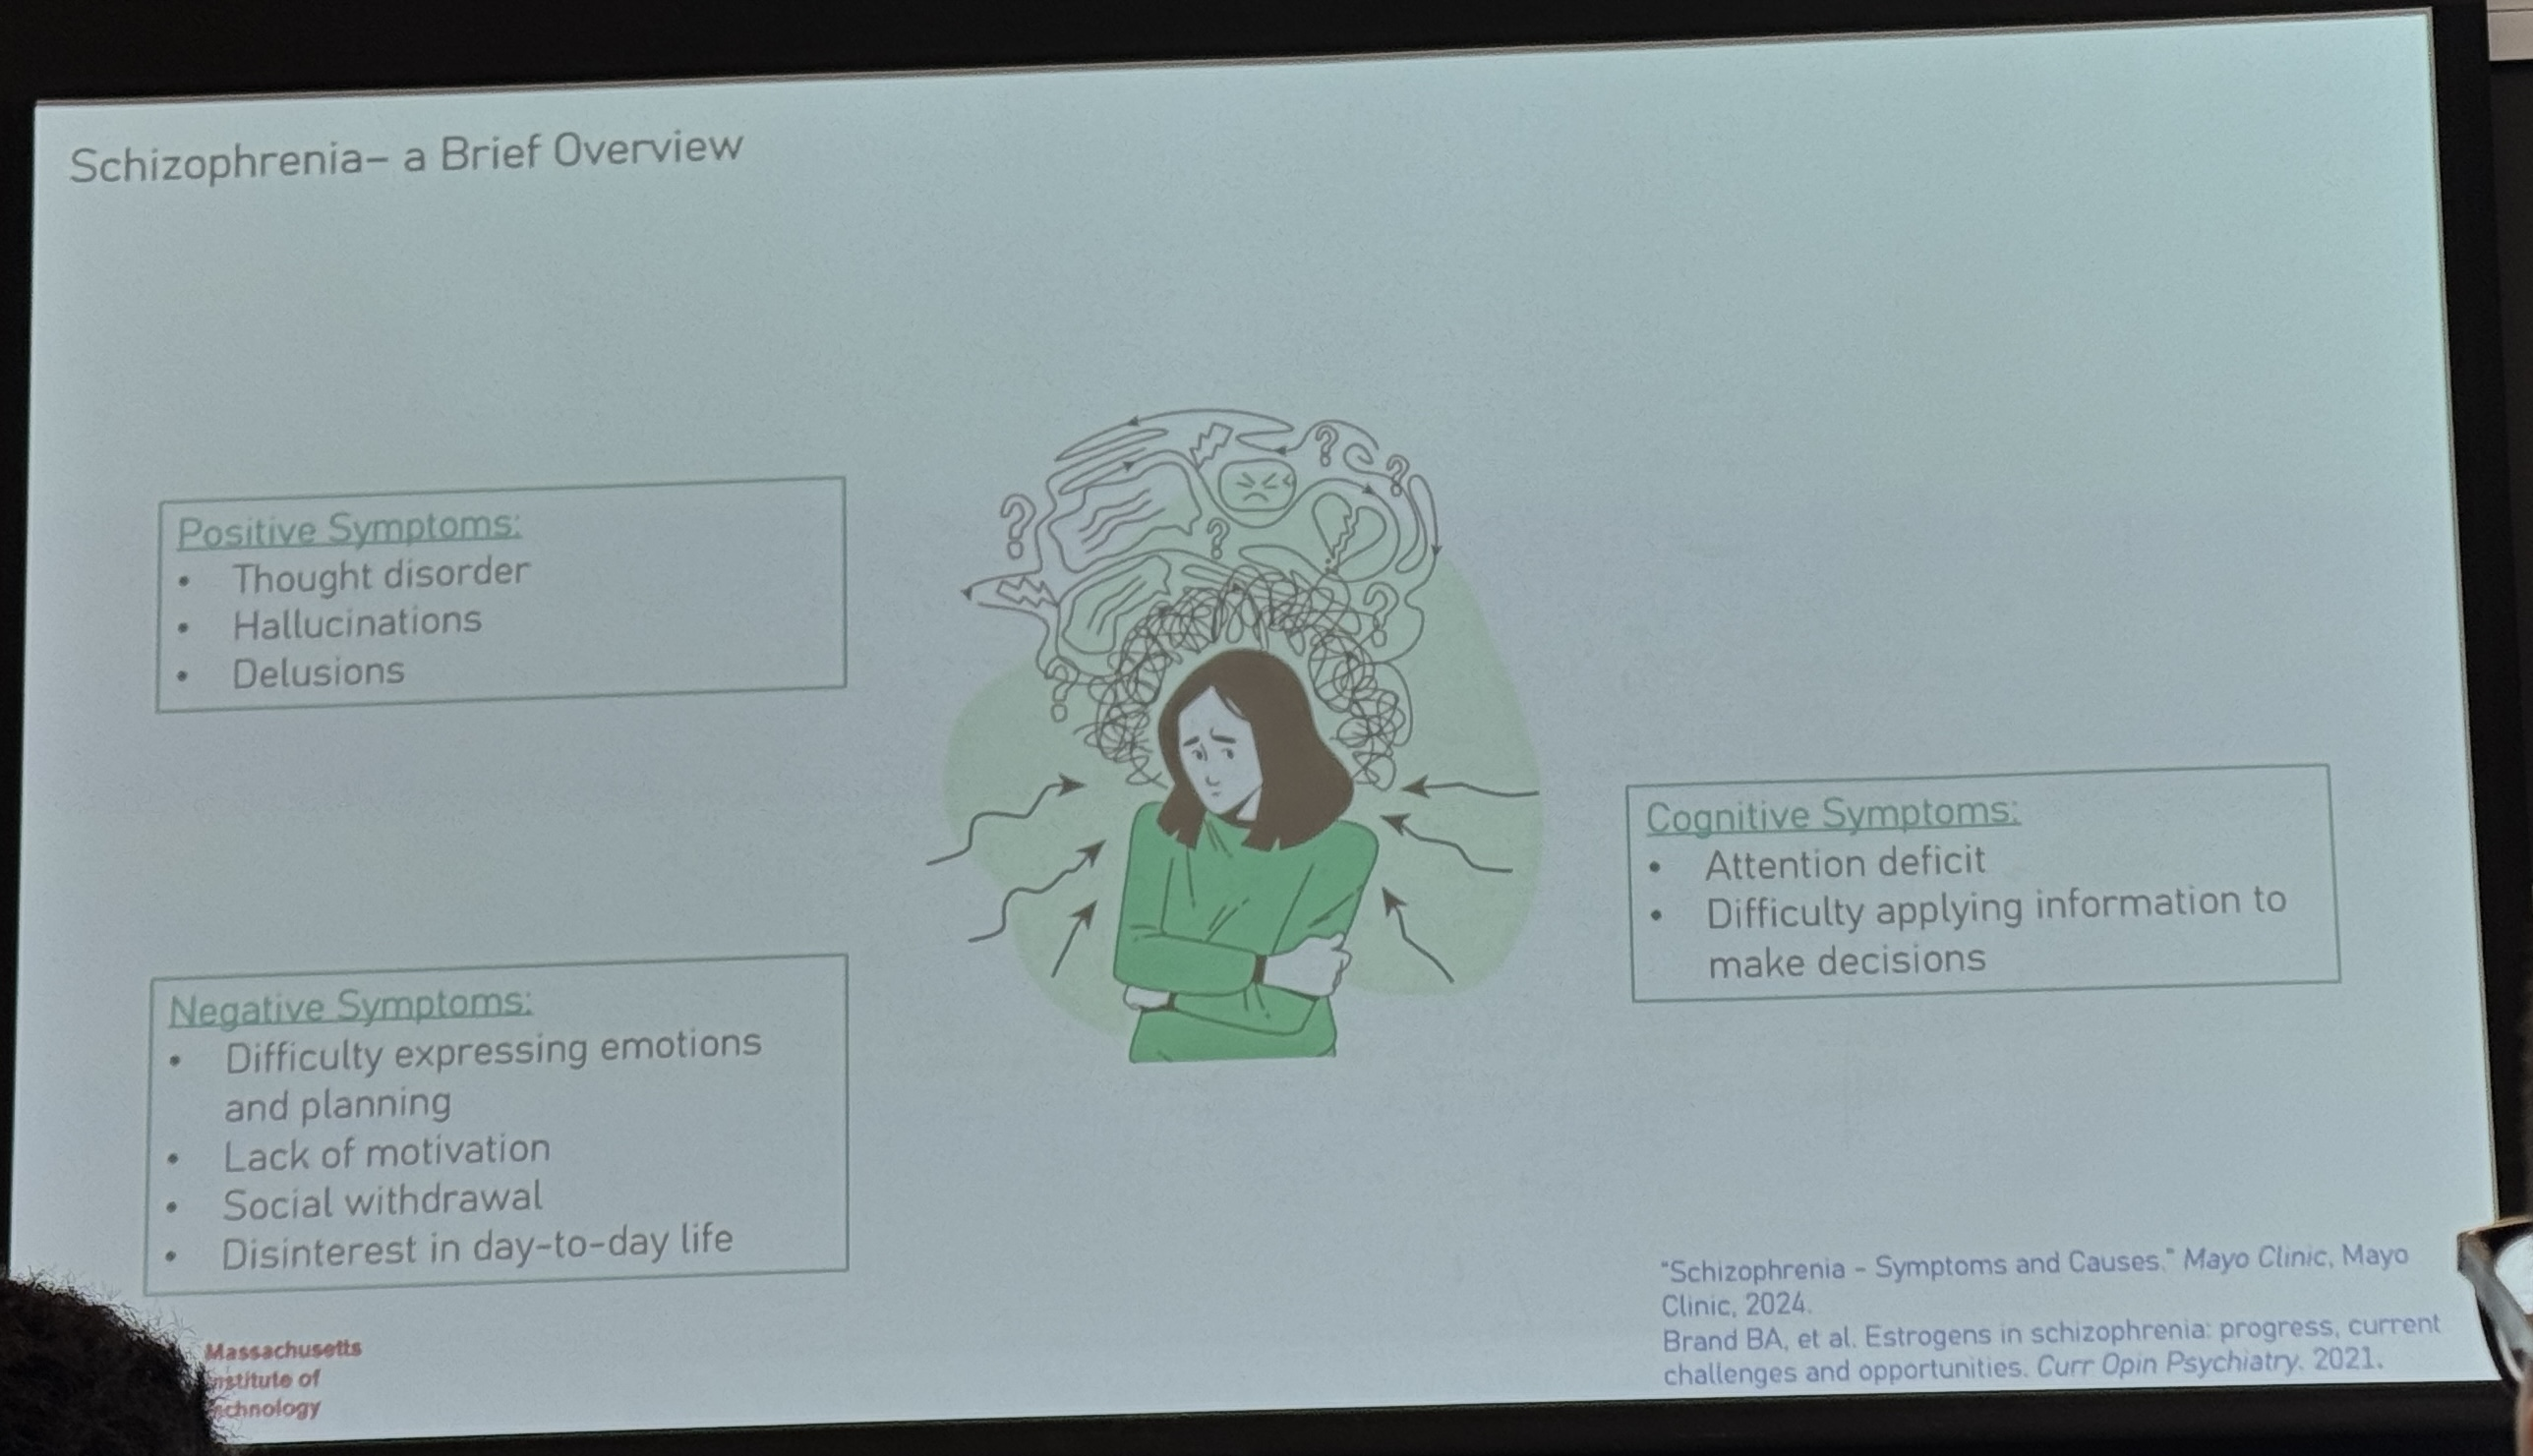
\includegraphics[width=0.7\linewidth]{PresElizabeth.JPG}
        \caption{Elizabeth's graphic design.}
        \label{fig:PresElizabeth}
    \end{figure}
    \begin{itemize}
        \item Cobenfy: Combination drug of xanomeline and trospium chloride.
        \item Graphic design: Boxes around an image to identify different aspects. Hard lines, good font, and color are all useful, though the color is a bit light and hard to read\dots
        \item \ce{TMSCN} is an alternate nucleophilic cyanide equivalent to \ce{KCN}.
        \item Thiadiazole synthesis from \ce{S2Cl2}, and a nitrile/amine. Mechanistically pretty complicated, per Steve.
    \end{itemize}
    \item Eva Bayer's (Harvard) presentation.
    \begin{itemize}
        \item Has radioactive \ce{{}^18F}.
        \item Higher image resolution (for PET) among competitors. Goes \emph{very specifically} to mitochondria.
        \item Good that a precursor was approved in pesticides, because it flushes out of humans super quickly, so no long-term toxicity. But hangs around long enough for imaging.
        \item Time really matters in the synthesis (it's 110 minutes, 35\% yield) because the \ce{{}^18F} decays so rapidly!
        \item You basically need a cyclotron on site to produce this stuff and get it into a patient ASAP.
    \end{itemize}
\end{itemize}



\section{Day 3 (15-21)}
\begin{itemize}
    \item \marginnote{3/18:}Jonah's presentation.
    \begin{figure}[h!]
        \centering
        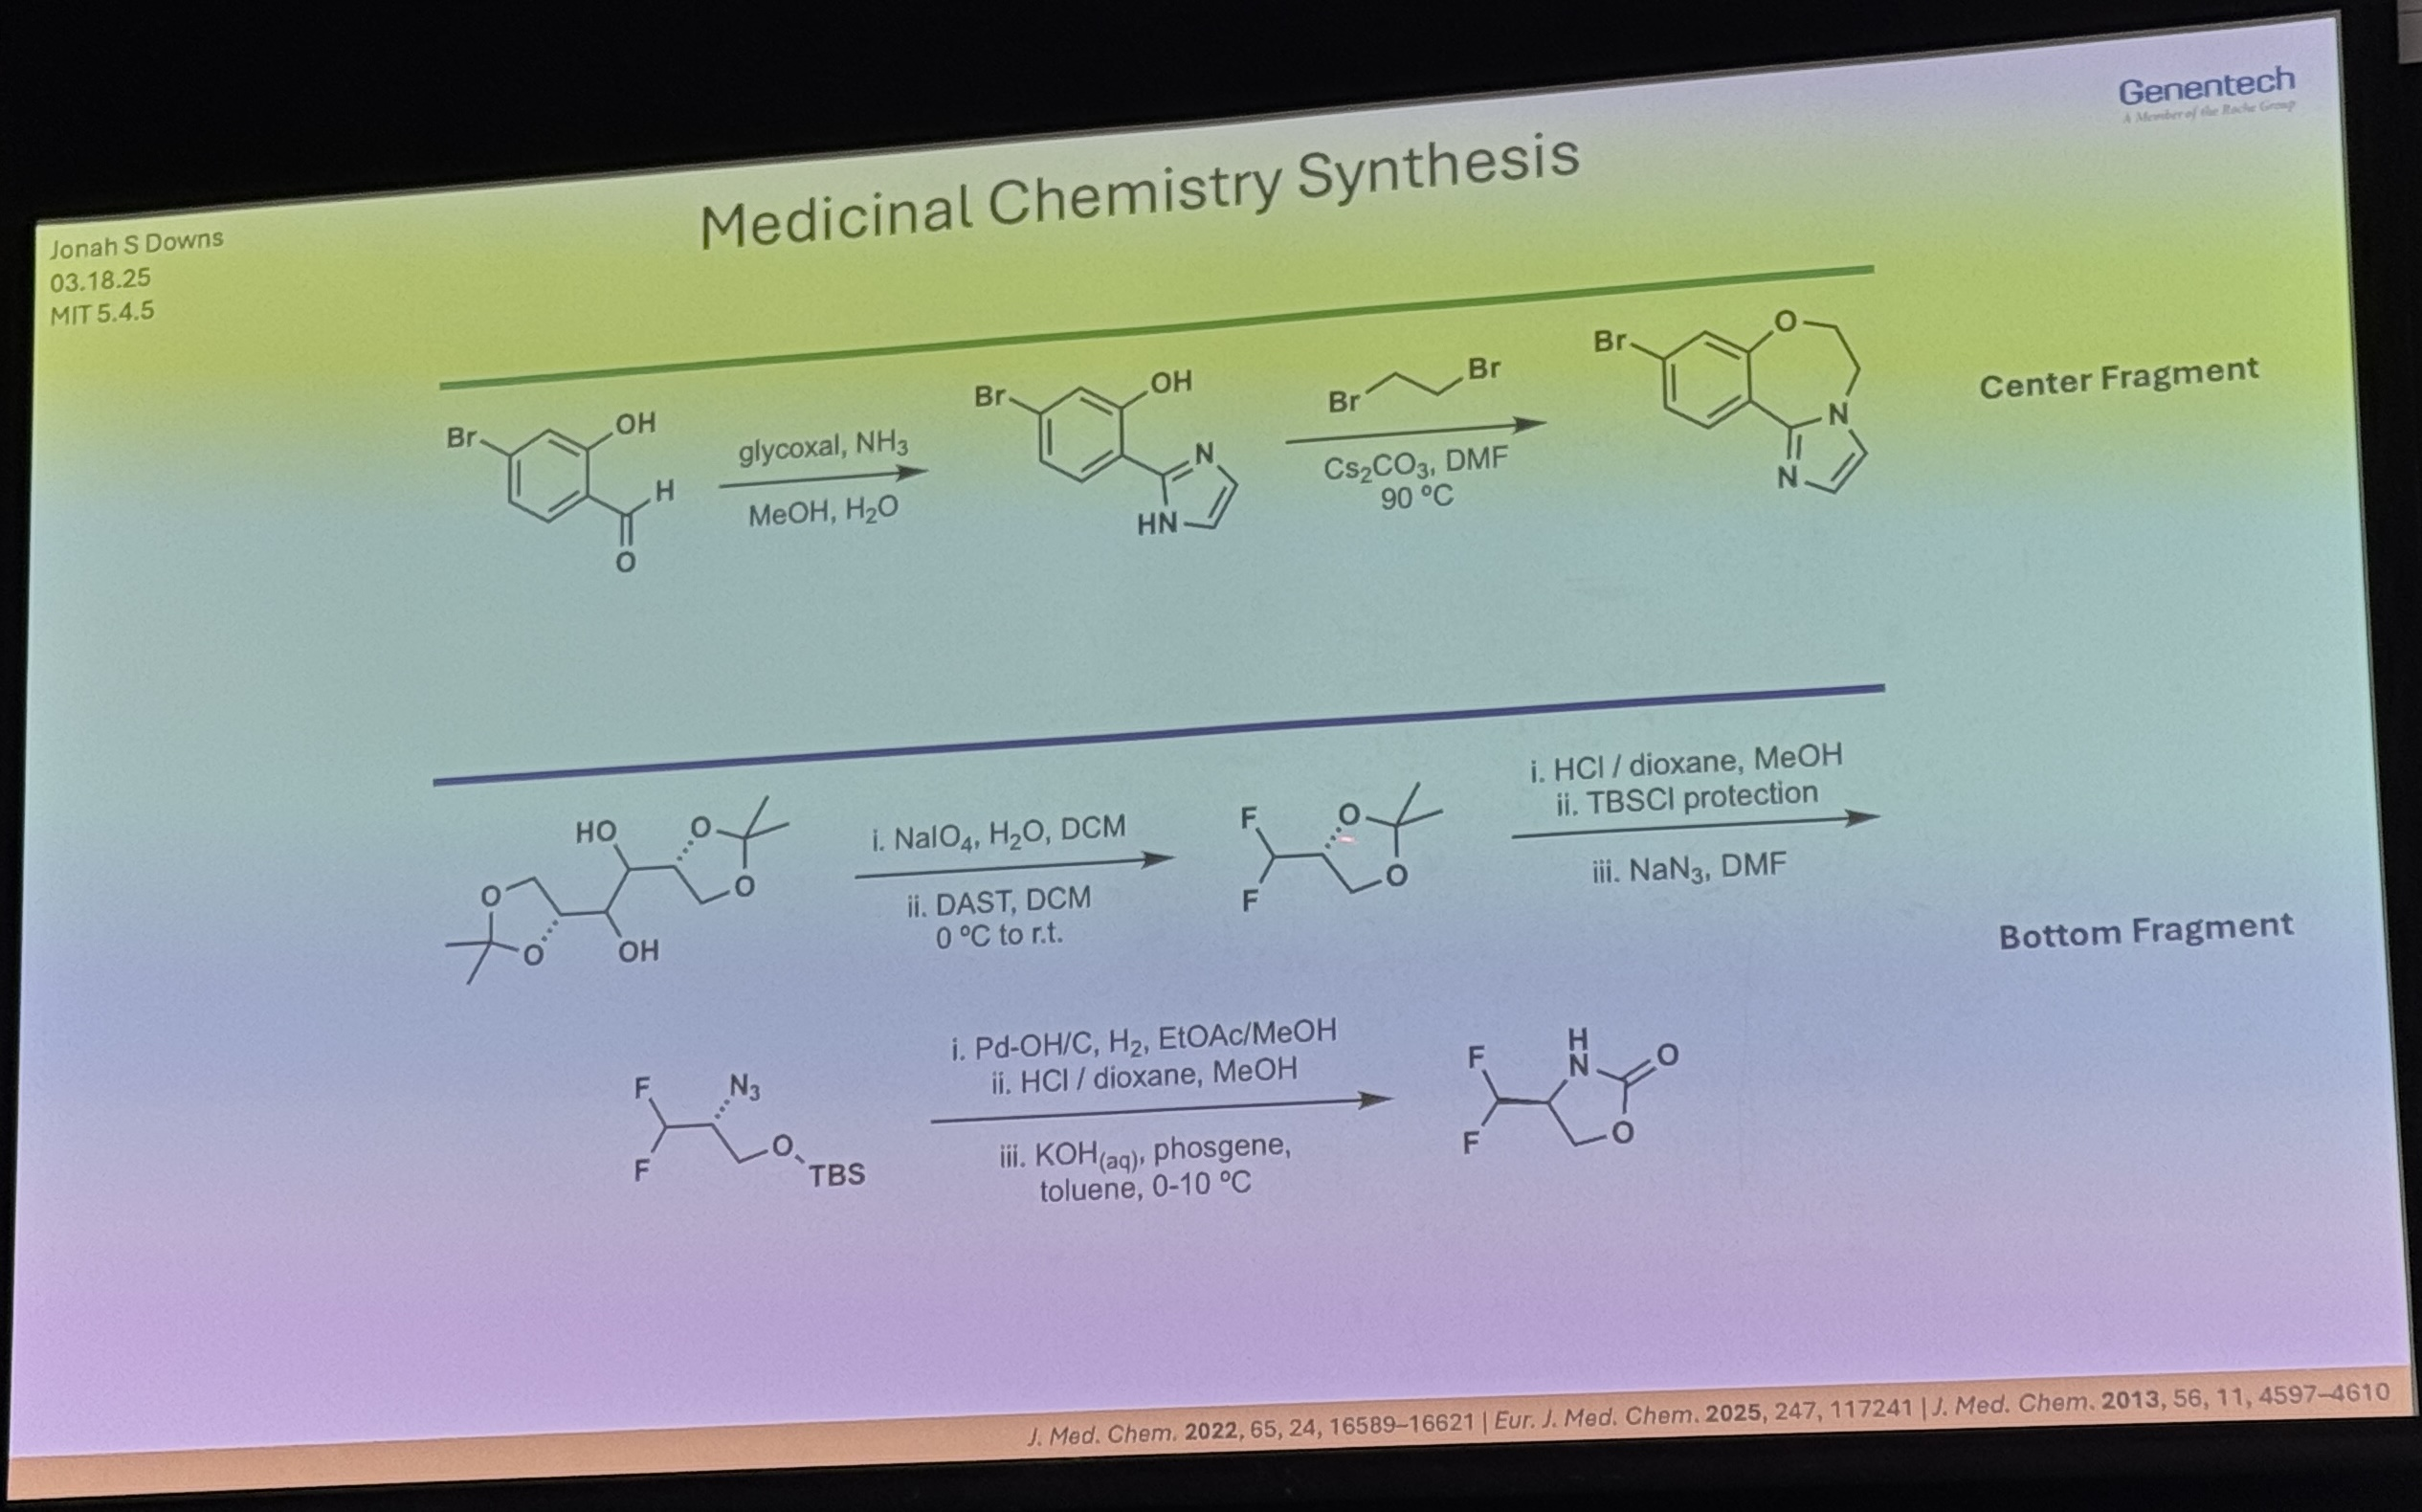
\includegraphics[width=0.7\linewidth]{PresJonah.JPG}
        \caption{Jonah's graphic design.}
        \label{fig:PresJonah}
    \end{figure}
    \begin{itemize}
        \item Itovebi.
        \item Buchwald-Ullmann-type cross-coupling; because Steve consults for Genentech, so they acknowledged him in the patent and publication.
        \item Graphic design.
        \begin{itemize}
            \item Different colored lines to separate different fragment syntheses.
            \item Colored bar at bottom with citations.
        \end{itemize}
    \end{itemize}
    \item Rachel's presentation.
    \begin{figure}[h!]
        \centering
        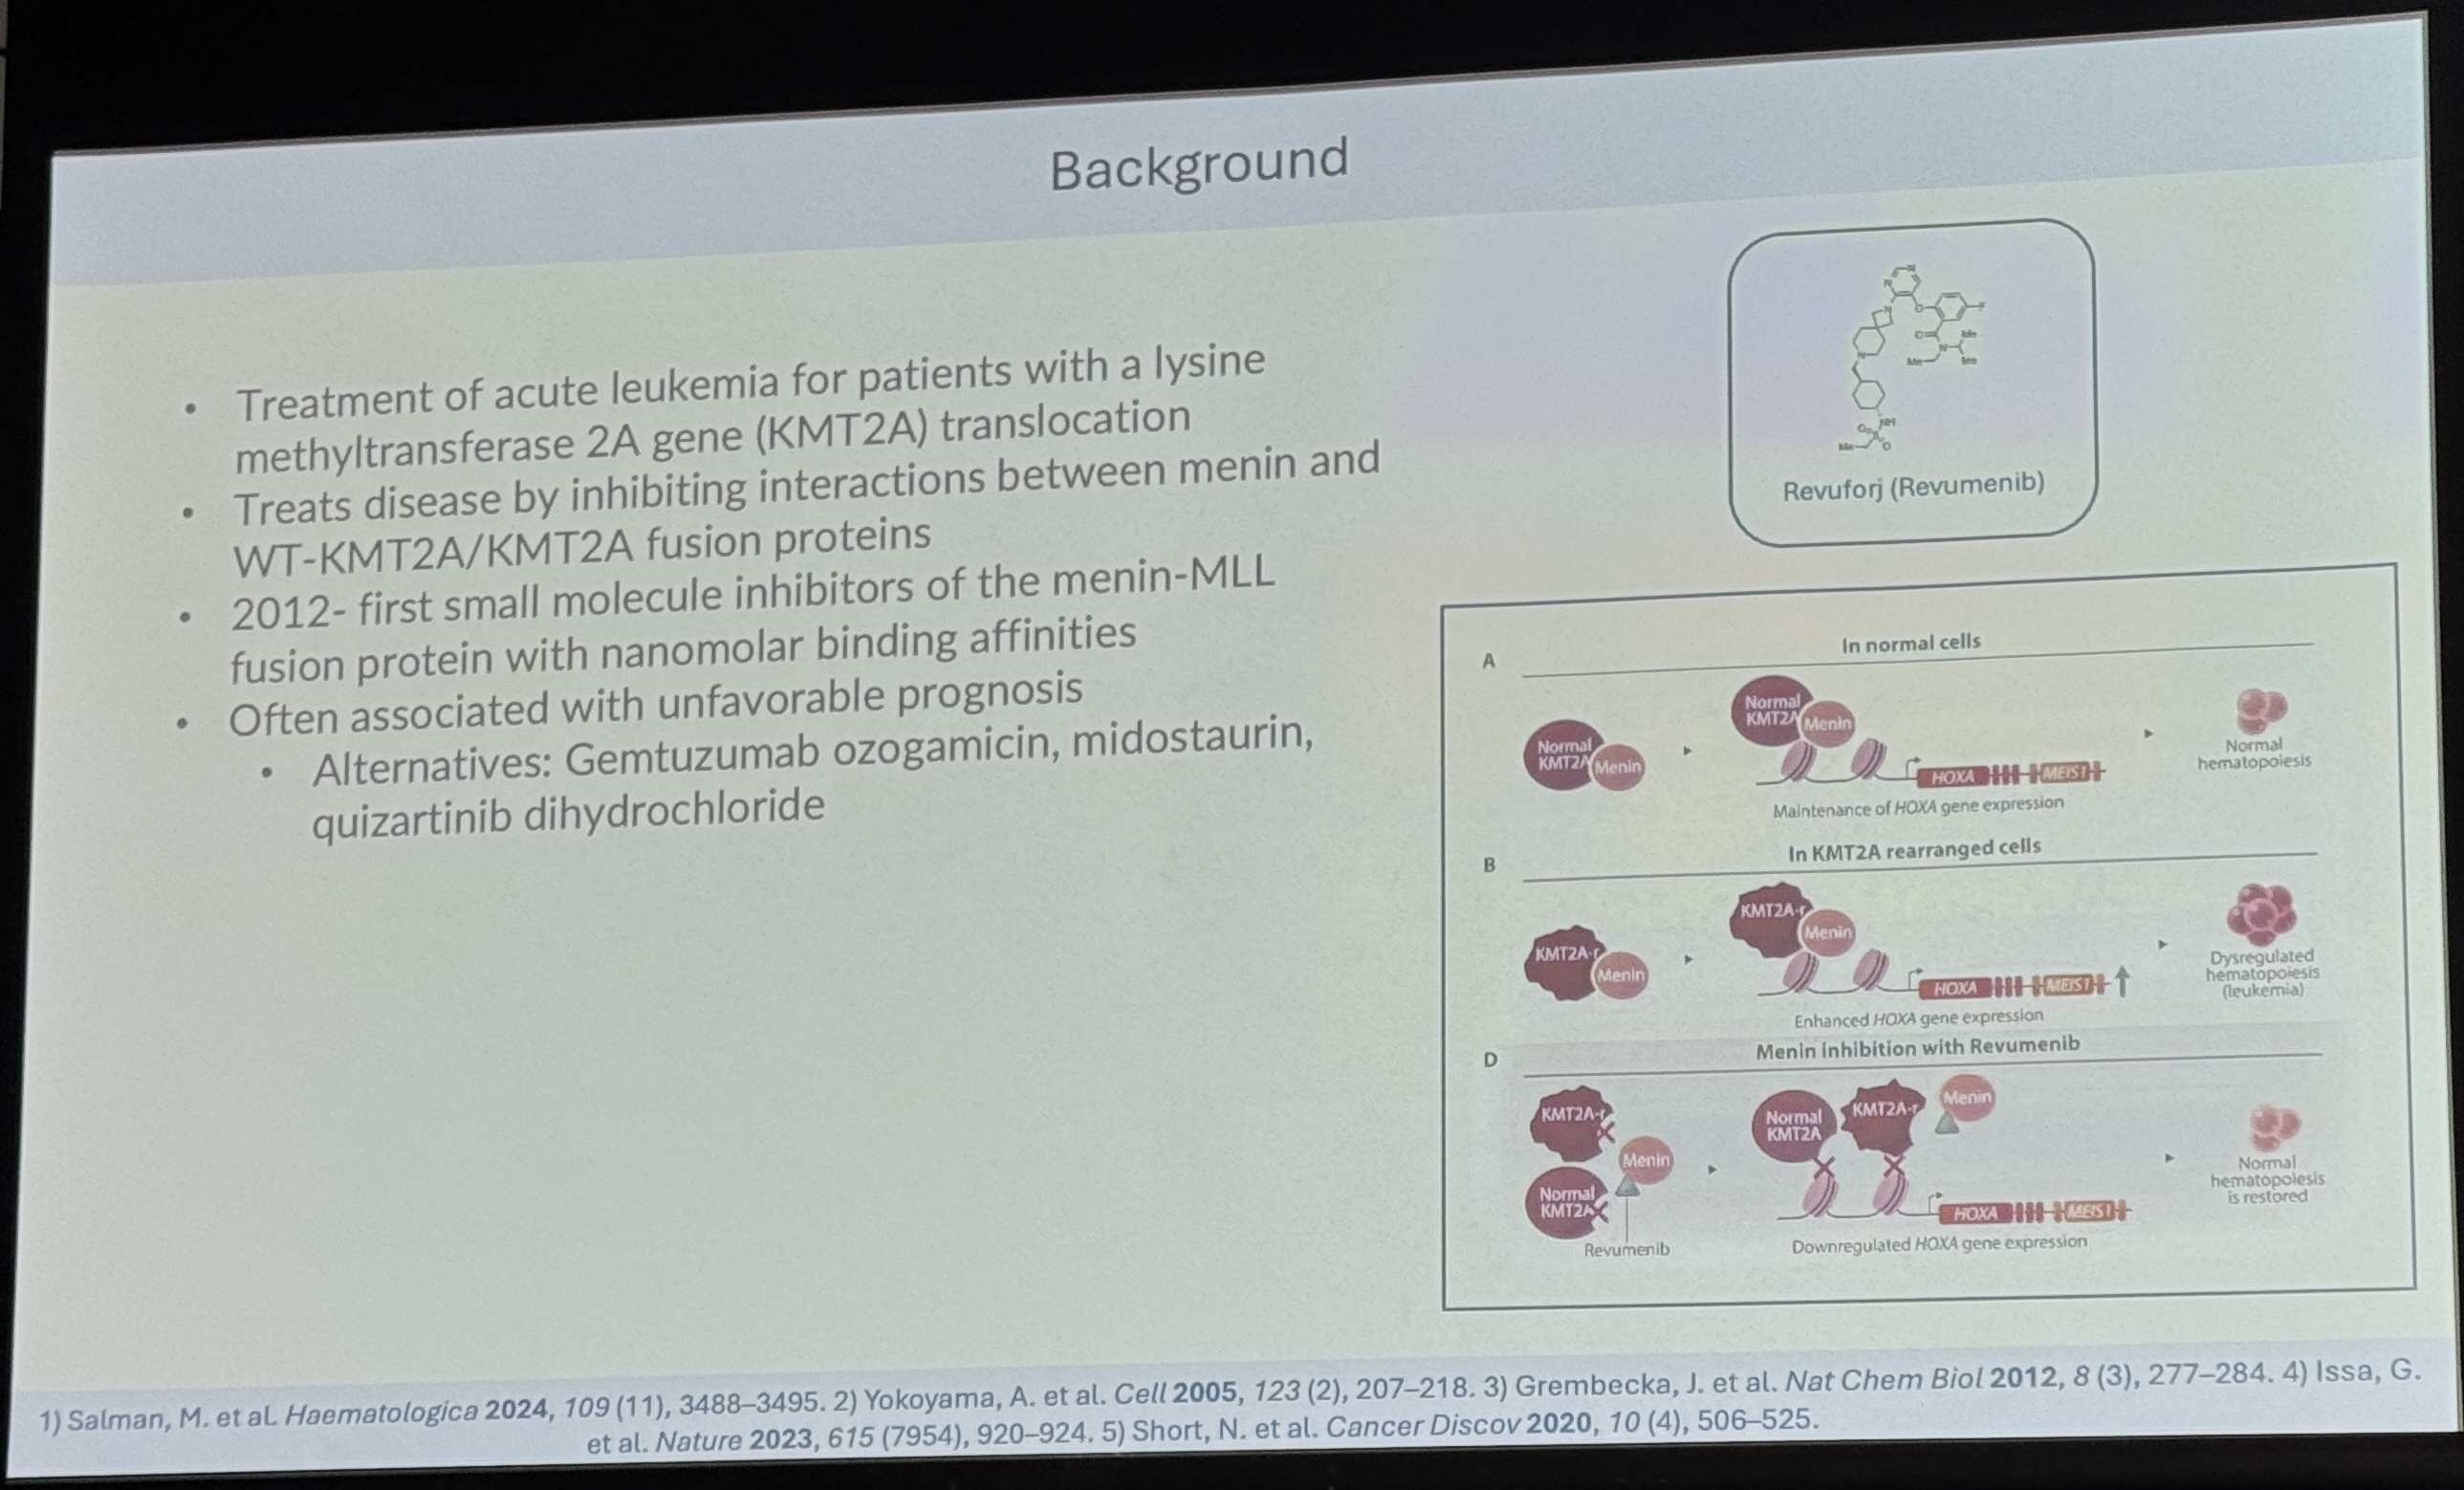
\includegraphics[width=0.7\linewidth]{PresRachel.JPG}
        \caption{Rachel's graphic design.}
        \label{fig:PresRachel}
    \end{figure}
    \begin{itemize}
        \item Revuforj.
        \item Graphic design.
        \begin{itemize}
            \item Also has colored bar at bottom with citations, matched by colored title bar at top. Bottom bar grows and shrinks if 2nd line is needed; font size is fixed.
        \end{itemize}
        \item There are known procedures for taking \emph{N}-oxides and going directly to substitution without going through the 2-chloro derivative with \ce{POCl3}.
    \end{itemize}
    \item Christina's presentation.
    \begin{itemize}
        \item Attruby.
    \end{itemize}
    \item Frank's presentation.
    \begin{itemize}
        \item Crenessity.
        \item Synthesis on hundreds of kilograms scale.
        \item Hydroxyls are sometimes incorporated so that you can make a prodrug; they're good linkers, like with JJ!
    \end{itemize}
    \item Nicol\'{a}s Manno's presentation.
    \begin{itemize}
        \item Ensartinib.
        \item Drew an auxiliary reaction scheme on the board in no time flat!
    \end{itemize}
    \item Ismael Wane's presentation.
    \begin{itemize}
        \item Zavzpret.
        \item \textbf{Jeffery modification} of the Heck reaction (ligand free, but often limited to aryl chlorides).
        \item DuPhos used for asymmetric hydrogenation.
        \begin{itemize}
            \item Developed by Mark Burk at DuPont.
        \end{itemize}
        \item Dianion cyclizes.
        \item \textbf{Erlenmeyer synthesis} (with Hippuric acid).
    \end{itemize}
    \item Andrew Yue's presentation.
    \begin{itemize}
        \item Graphic design.
        \begin{itemize}
            \item Highlights the bonds that are formed, and it does help.
            \item It is also very important to conserve the relative orientation of moieties between steps as much as possible!
            \item Animation idea: When you have to do a synthesis across multiple slides, have everything but the last compound fade away, then have the last compound slide to the top-left corner of the next slide.
        \end{itemize}
        \item \textbf{Molander salts} in a Suzuki-type coupling.
        \item \textbf{Chiral supercritical fluid chromotography} (chiral SFC) can resolve atropisomers.
        \item Fluoride limits reactor size (it etches glass and stainless steel); you have to use \textbf{Hastelloy reactors}, which are much more expensive.
        \item Steve: This has got to be an incredibly expensive moleucle. There's much less price pressure as oncology drugs because people will pay to save their lives.
    \end{itemize}
    \item 2nd exam on Thursday.
    \begin{itemize}
        \item 2023 practice exam is a final exam.
        \item 2024 exam is more like this one.
        \item Try to be here a bit before 9:00 AM.
    \end{itemize}
    \item Notes on presentations.
    \begin{itemize}
        \item It's harder to do biocatalytic processes in discovery, but they're great in long-term process routes.
    \end{itemize}
\end{itemize}




\end{document}